
\chapter{試料作成,ST-FMR測定及びイオン液体を用いた電気化学エッチング方法}\label{chap:making}
本研究ではNi$_{81}$Fe$_{19}$/Pt二層薄膜構造の試料をST-FMR測定のための電極と共に用意し,その試料におけるNi$_{81}$Fe$_{19}$をイオン液体を用いてエッチングしながらST-FMR測定を行なった.試料のバー及び電極構造はレーザー描画法とリフトオフ法を用いた.金属薄膜の成膜は全てスパッタリング法を用いた.
本章では本研究で用いた試料作成方法とST-FMR測定による電流-スピン軌道トルク生成効率の定量方法,さらにイオン液体を用いた電気化学エッチングの詳細について述べる.

\section{試料設計及び作成方法}
\subsection{スパッタリング法を用いた金属薄膜の成膜}
本研究で用いた金属薄膜試料は全てレーザー描画法により作成した微細構造マスクを用いて成膜した.
試料を成膜した基板はタングステンカーバイドペンにより1.6 cm$\times$1.6 cmの大きさにカットした熱酸化Si基板(Si: 400 $\mu$m,SiO$_2$: 100 $\mu$m)である.金属薄膜を成膜前にSiO$_2$基板をアセトン,エタノールの溶液中に入れ,それぞれ30分間,10分間超音波洗浄を施した.エタノール洗浄後にはN$_2$ガンによりN$_2$ガスを基板上に吹きかけ基板上に残留しているエタノール及び有機物を除去した.
本研究では強磁性金属としてNi$_{81}$Fe$_{19}$,常磁性金属としてPt,電極としてAu/Tiの金属薄膜をそれぞれスパッタリング法により成膜した.ただし,Auに関してはSiO$_2$基板上に単体での均質な薄膜を成膜することが困難であったので(アイランド状に粒を作ってしまう),最初にSiO$_2$基板とAuの接着層としてTiをスパッタリング法により成膜しそのTi上にAuを成膜した.
成膜時の条件を表\ref{tb:deposite condition}に示す.
成膜は最初にArガスの圧力を1 Pa程度に調節した状態で直流(DC)電源で電力を0.1 kWにしてプラズマを発生させた.この状態で高周波(RF)電源を表\ref{tb:deposite condition}のような電力条件にしてつけ,そしてプラズマが安定したところでDC電源をきる.RF電源に切り替えた後に成膜条件のAr気圧となるよう排気の量を調節した.

Ni$_{81}$Fe$_{19}$/Pt二層薄膜及び電極の作成に関して利用したレーザー描画法及びリフトオフ法について次に記述する.

\begin{table}[htbp]
 \caption{金属薄膜成膜時のスパッタリング法の成膜条件.}
 \begin{center}
  \begin{tabular}{cccc}\toprule
  	金属	&	Arガスの気圧	&	電源電力		&	rate (nm/sec)	\\	\hline
	Pt		&	0.23 Pa			&	RF  60 W		&					\\
	Ni$_{81}$Fe$_{19}$ &	0.24 Pa			&	RF  50 W		&	
	\\
	Ti  &   0.24 Pa   &    RF 50 W   &
	\\
	Au  &  0.24 Pa   &   RF 50 W   &   
						\\	\bottomrule
  \end{tabular}
 \end{center}
 \label{tb:deposite condition}
\end{table}

\begin{figure}[htbp]
 \begin{center}
  %\includegraphics[width=85mm]{metalmask.eps}
 \end{center}
 \caption{(a)Ni$_{81}$Fe$_{19}$/Pt二層薄膜構造作成に用いたレーザー描画法における描画パターン,(b)強磁性細線構造作成に用いた電子線描画法における描画パターン及び(c)電極作成に用いたレーザー描画法における描画パターン.
 }
 \label{maskpattern}
\end{figure}





\subsection{レーザー描画法及びリフトオフ法を用いたST-FMR測定系の作成}
レーザー描画法は試料基板に塗布した有機物の膜(レジスト)を感光させ,パターンを作成する方法である.
本研究ではレーザー描画法及びリフトオフ法により目的の試料パターン構造及び電極を作成した.最初にレーザー描画法及びリフトオフ法を用いたバー構造の作成過程について以下に示す.

\begin{figure}[htbp]
 \begin{center}
  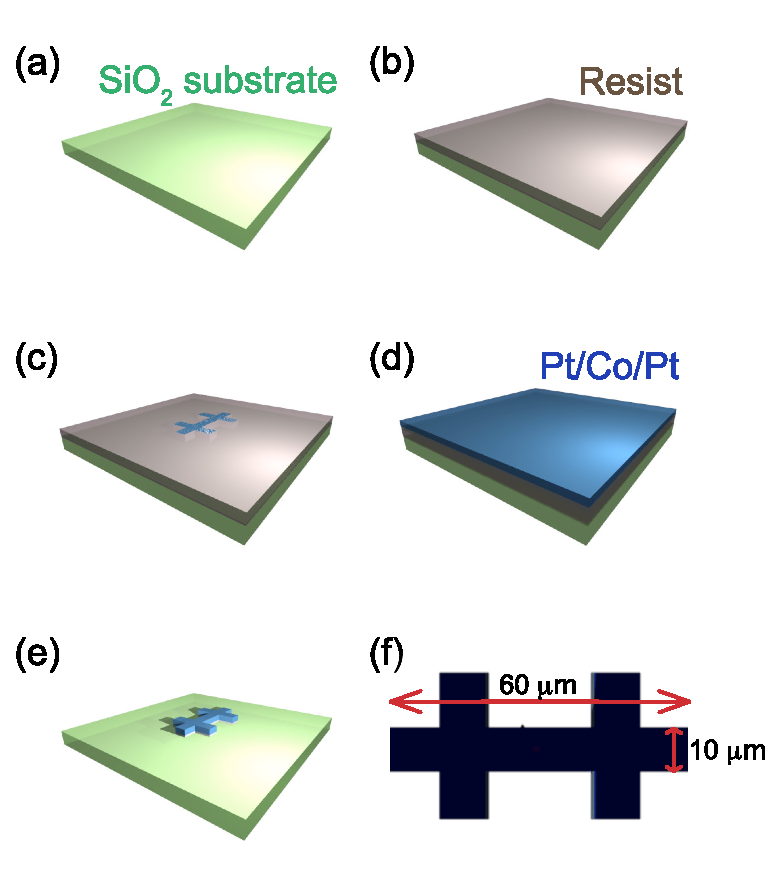
\includegraphics[width=100mm]{images/Making_samples.eps}
 \end{center}
 \caption{(a)-(e)レーザー描画法とリフトオフ法によるNi$_{81}$Fe$_{19}$/Pt二層薄膜構造の作成過程.(a)-(c)に示すようにレーザー描画法を用いてホールバーレジストマスクパターンをSi基板上に作成し、(d)に示すようにNi$_{81}$Fe$_{19}$/Pt層を成膜した後、レジスト層をリフトオフ法によって剥離した(e)。この後同様の流れで電極パターンとしてAu/Tiを成膜した.(f)ホールバーのパターンの大きさを示した.}
 \label{Making_samples}
\end{figure}

熱酸化Si基板をタングステンカーバイトペンを用いて1.6 cm$\times$1.6 cmの大きさにカットした後に超音波洗浄器を用いてアセトンで30分間洗浄し,さらにエタノールにより10分間洗浄してからN$_2$ガンによりエタノールを吹き飛ばし乾燥させた(図\ref{Making_samples}(a)).
次にスピンコーターに洗浄した基板を乗せ,そこにネガ型レジスト溶液(ZPN1150-90)を塗布した.ここで用いたネガ型レジストとは,露光されると感光部分の現像液に対する溶解性が減少し,現像後に露光部分が残るものである.
スピンコーターの条件はまず回転速度500 rpmで5秒間回転させた後,3000 rpmで30秒間回転させた.これにより基板上にレジストを均一に塗布した.その後,$100\rm\ ^{\circ}C$に加熱されたホットプレートで基板を90 秒間ベーキングし,レジスト薄膜を成膜した(図\ref{Making_samples}(b)).
レジスト成膜後はレーザー描画装置を用いてパターン以外の部分に紫外線を照射しパターンをレジスト上に作成した.このときのレーザー描画装置の条件はdefocusが-6でexposure timeが24 msで行った.



レーザー描画した後,基板を$100\rm\ ^{\circ}C$に設定したホットプレートに1分間乗せてポストベークし,現像液(AZ 300MIF DEVELOPER(2.38\%))に42秒浸し,さらにレジストを除去するために純水に1分程度つけることで露光されていない部分を除去した(図\ref{Making_samples}(c)).これによりレジストマスクパターンが完成した.そこへスパッタリング装置を用いて常磁性金属Ptを10 nmを成膜し,その上にさらに強磁性金属Ni$_{81}$Fe$_{19}$を8 nmを成膜した(図\ref{Making_samples}(d)).
成膜後,剥離液であるアセトンに試料をつけ,レジストマスクを剥離した.するとレジストのなかった部分だけが基板上に残り,Ni$_{81}$Fe$_{19}$/Ptのバー上の試料が作成できた(図\ref{Making_samples}(e)).
このようにレジストマスクを作成し,そこへ成膜し,レジストマスクを除去することで所望のパターンを形成する方法をリフトオフ法という.
このホールバーは微小なため,
同様の過程のレーザー描画法により図のような電極パターンのレジストマスクを作成した.
電極はAuを使用したが,金単体ではSi0$_{2}$基板上に安定的に着かず剥がれてしまうのでTiを接着層としてまず成膜しその上にAuを成膜し電極を作成した.その結果が図\ref{madehallbar}である.

\begin{figure}[htbp]
 \begin{center}
  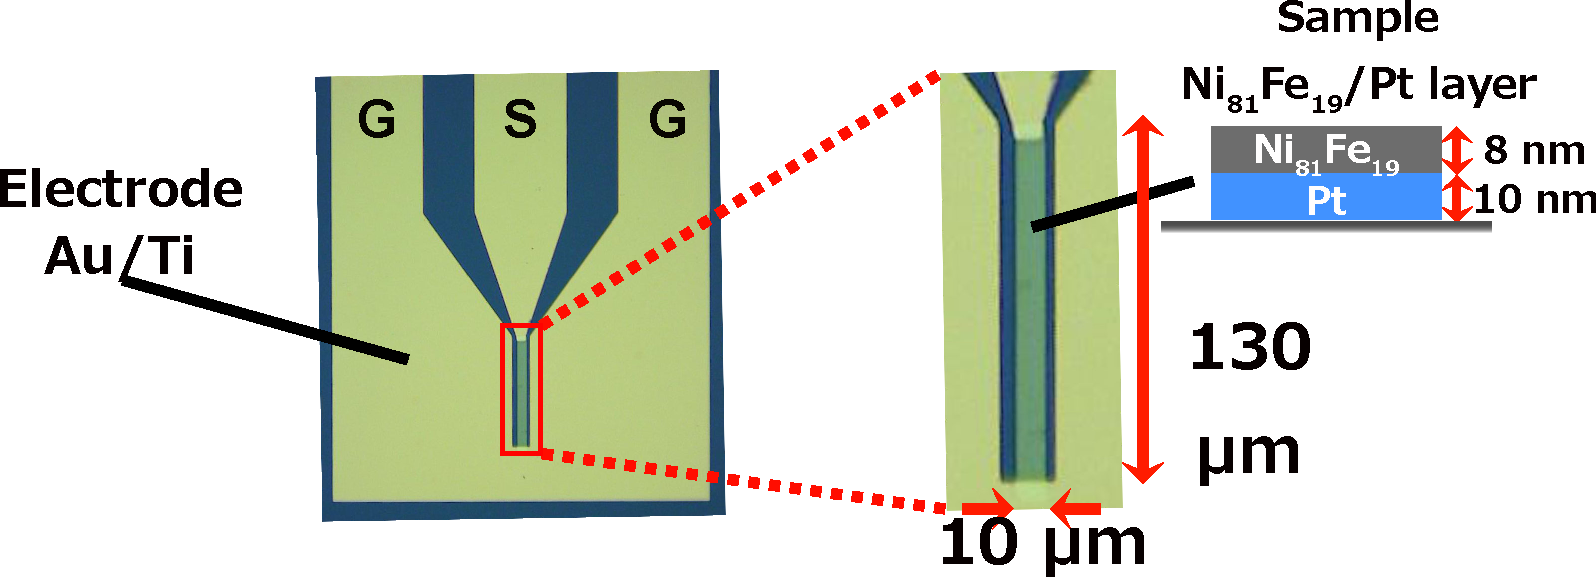
\includegraphics[width=150mm]{images/STFMRpicture.pdf}
 \end{center}
 \caption{作成したホールバーのレーザー顕微鏡図及びレーザー顕微鏡図を拡大した図.右側の細長いバー状の部分がNi$_{81}$Fe$_{19}$/Ptである.}
 \label{madehallbar}
\end{figure}

実際は図\ref{madehallbar}のホールバーおよび電極が1.6 cm$\times$1.6 cmの熱酸化Si基板上に6つ作成できるよう設計図を作成した.
以上のようにしてNi$_{81}$Fe$_{19}$/Pt二層薄膜ホールバー構造及び電極が完成した.


\section{ST-FMR測定を用いた電流-スピン軌道トルク変換効率の定量}\label{FMR_uniform}

この章ではST-FMR測定を用いた電流-スピン軌道トルク生成効率の定量方法について述べる.
ST-FMR測定とは磁化の歳差運動によって強磁性体の抵抗が磁気抵抗効果によって時間依存した変化が起きることを利用した技術である.試料に時間変化する電流$I\cos (\omega t)$を流したとき,その電流によって強磁性体にトルクが与えられその電流と同じ周波数で強磁性体の抵抗が変化する.この電流及び抵抗変化から試料においてDC電圧が生じることになる.この定常電圧$V_{\rm DC}$によって時間の運動を検出することができる.この$V_{\rm DC}$が生じる効果を視覚的に記述するとFig.\ref{fig:frequencymix}のように描ける.

\begin{figure}[htbp]
 \begin{center}
  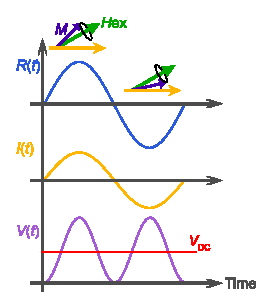
\includegraphics[width=8cm]{images/frequencymix.eps}
 \end{center}
 \caption{$V_{\rm DC}$の生じる原理.歳差する磁化$M$が時間変化する抵抗$R(t)$が生じその周波数はその磁化を歳差させている電流の周波数と同じである.それらの掛け合わせによって電圧$V(t)$が発生し,実際の測定においてはその平均値である定常電圧$V_{\rm DC}$を測定する.}
 \label{fig:frequencymix}
\end{figure}

\subsection{測定系について}

\begin{figure}[htbp]
 \begin{center}
  \includegraphics[width=85mm]{hallbar.eps}
 \end{center}
 \caption{本研究の測定系}
 \label{fig:setup}
\end{figure}
本研究の測定系は図\ref{fig:setup}のようになっている.試料に交流電流$\Delta I\sin\omega t$を流し,電磁石によって外部磁場を試料の面内方向に与える.このときのホール電圧$V_{XY}$は
\begin{eqnarray}
V_{XY} = V_{0}+V_{\omega}\sin\omega t + V_{2\omega}\cos\omega t
\label{eq:Vxy}
\end{eqnarray}
となる.
このホール電圧$V_{XY}$からロックインアンプを用いて高調波Hall電圧$V_{\omega}$と$V_{2\omega}$を測定した.高調波Hall電圧とは流した交流電圧の周波数の整数倍となる周波数で振動するHall電圧のことを指している.

これらの高調波Hall電圧の1次成分$V_{\omega}$と2次成分$V_{2\omega}$からスピン軌道トルクの有効磁場を算出でき,その関係は以下のようになっている\cite{yang2015layer,kim2013layer}.このプレーナーホール効果による電圧が異常ホール効果による電圧に対して微小であるときを想定している.
\begin{eqnarray}
\Delta H_{T(L)}=-2\frac{\partial V_{2\omega}}{\partial H_{T(L)}}\biggl/\frac{\partial^{2} V_{\omega}}{\partial^{2} H_{T(L)}}
\label{eq:torque}
\end{eqnarray}
ただし$H_{T(L)}$は外部磁場を表している.外部磁場を電流に対して平行にかけると$\Delta H_{T}$が測定でき,垂直にかけると$\Delta H_{L}$が測定できる.$\Delta H_{T}$,$\Delta H_{L}$は磁化にかかる有効磁場で添え字のTやLは電流に対して平行か垂直かを表している.

試料が面直磁化容易膜(面直磁化膜)である場合,有効磁場$\Delta H_{T}$はfield-likeトルクを,$\Delta H_{L}$はdamping-likeトルクを起源としているとわかっている\cite{yang2015layer}.そこで,本研究ではこの有効磁場$\Delta H_{T(L)}$の変化をスピン軌道トルクの変化として扱うことにする.

\subsection{スピン軌道トルクの導出}


%以上の計算はプレーナーホール効果による電圧を無視して考えているため電流と磁場の方向によって$\Delta H_{T(L)}$を分離することができている.プレーナーホール電圧による寄与を無視するということは電流に対して平行な磁化の動きに対応する電圧を無視するということを意味する.実際の磁化の動きは図\ref{harmonicFig}のように表せる.垂直磁化膜の磁化は図\ref{harmonicFig}(a)のような平衡状態にある.そこに交流電流を流し外部磁場を印加すると図\ref{harmonicFig}(b)(c)のように磁化が動く.


%図(\ref{harmonicFig})において(b)では$\Delta H_{T}$によって,(c)では$\Delta H_{L}$によってプレーナーホール電圧が誘起されるはずである.









\subsection{イオン液体を利用した電気化学エッチングの方法}

イオン液体

%本研究では磁化ダイナミクス励起及び磁化ダイナミクスの解析に電子スピン共鳴(Electron Spin Resonance: ESR)装置を用いた。電子スピン共鳴装置は測定試料に固定角周波数$\omega$のマイクロ波を照射し、外部直流磁場$H$を掃印した際の
%試料によるマイクロ波吸収を測定するものである。以下では電子スピン共鳴装置により得られる強磁性共鳴スペクトルと磁化ダイナミクスの関係を示す。

%強磁性体中の磁化ダイナミクスは式(\ref{LLG})のLLG方程式に従う。式(\ref{LLG})は磁化が有効磁場$\bm{H}_\text{eff}$を軸として歳差運動を行い、スピン角運動量やエネルギーを散逸して$\bm{H}_\text{eff}$方向に緩和することを示している。
%磁化歳差運動の角周波数と等しい角周波数を持つマイクロ波を照射すると、磁化はマイクロ波からエネルギーを吸収して減衰することなく歳差運動を続ける。これが強磁性共鳴である~\cite{Chikazumi}。


%強磁性共鳴によるマイクロ波の吸収スペクトルから、磁化ダイナミクスを支配するパラメータの一つである緩和定数$\alpha$を実験的に求めることが可能である\footnote{$\alpha$は歳差運動の緩和時間$\tau$を定めるパラメータである。
%LLG方程において有効磁場$\bm{H}_\text{eff}$が$z$方向を向いている場合を考える。
%歳差運動の振動成分$m_x$, $m_y$の解を$(m_x,\; m_y)=m_0 e^{-t/\tau}(\cos\omega t,\; \sin\omega t)$とする。
%$\tau$は歳差運動の緩和時間である。$M_s^2=m_x^2+m_y^2+M_z^2$から$M_z=M_s\left(1-(m_0/M_s)^2 e^{-(2t/\tau)}\right)^{1/2}$となり、時間経過によって$M_z=M_s$に緩和する。また$m_x$, $m_y$をLLG方程式に代入すると
%$d M_z/dt=(\alpha/M_s)m_0^2\omega e^{-2t/\tau}$
%が得られる。この2式より$
%\alpha\tau\omega=\left(1-(m_0/M_s)^2e^{-2/\tau}\right)^{-1}$
%となり、微小振動$(m_0/M_s)^2\ll 1$の範囲では緩和時間$\tau$と緩和定数$\alpha$の間に
%\begin{equation}
%\tau\simeq 1/\alpha\omega\nonumber
%\end{equation}
%の関係がある。
%}。
%この概要を以下に示す。
%外部直流磁場$H$とマイクロ波磁場$h$を考え$\bm{H}=(h\cos \omega t,h\sin \omega t,H)$とする。複素磁化率$\chi=\chi'-i\chi''$を導入すると、同位相応答の磁化$M'$と$\pi /2$位相遅れの磁化$M''$の$y$成分は
%$M_y'=\chi 'h\sin \omega t$及び$M_y''=-\chi ''h\cos \omega t=\chi ''h\sin (\omega t-\pi /2)
%$となる。強磁性試料によるマイクロ波吸収は単位時間あたりの磁気的エネルギーの変化分$H(dM/dt)=Hd(M'+M'')/dt$に対応するため、強磁性共鳴によるマイクロ波吸収量$I$は
%振動磁場一周期あたりのマイクロ波吸収の時間は$2\pi /\omega$であるので、全吸収量は
%\begin{eqnarray}
%I=\frac{\omega}{2\pi}\int^{2\pi/\omega}_0 \bm{H}\cdot\frac{d\bm{M}}{dt}dt
%=\frac{1}{2}\omega\chi'' h^2\label{absorption}
%\end{eqnarray}
%となり、複素磁化率の虚数成分$\chi''$に比例する。

%磁化率の虚数成分は強磁性薄膜面内に磁場を印加した場合
%\begin{equation}
%\chi '' = \frac{\alpha{M_s}\left( H_\text{FMR} + 4\pi {M_s} \right)  }{2\left( H_\text{FMR} + 2\pi {M_s}  \right)}\frac{\left(\omega/\gamma\right)}{ (H - {H_\text{FMR}})^2+\left(\alpha\omega/\gamma\right)^2}
%\end{equation}
%で与えられる\footnote{第\ref{formulation}章 式(\ref{chi3})参照}。ここで$H_\text{FMR}$は強磁性共鳴磁場を表す。従って式(\ref{absorption})より、共鳴磁場付近($H\approx H_\text{FMR}$)におけるマイクロ波吸収量$I$はローレンツ関数
%\begin{equation}
%I(H) = \frac{1}{4 } {M_s}  h^2\gamma\left(\frac{{ {{H_\text{FMR}} + 4\pi {M_s}}  }}{  H _\text{FMR}+ 2\pi {M_s} }\right)\frac{\alpha  (\omega/\gamma)^2}{ { {{(H - {H_\text{FMR}})}^2}+(\alpha \omega /\gamma)^2 } }\label{absorption2}
%\end{equation}
%となる。
%電子スピン共鳴装置では磁場変調によるロックイン法を用いているため、測定される吸収スペクトルは図\ref{FMR}に示すような式(\ref{absorption2})の微分形$dI(H)/dH$である。
%図\ref{FMR}に定義した微分吸収曲線のピーク間線幅$W$は式(\ref{absorption2})より
%\begin{equation}
%W=\frac{2\omega}{\sqrt{3}\gamma}\alpha \label{Wtoa}
%\end{equation}
%で与えられる。従って電子スピン共鳴装置を用いた強磁性共鳴によるマイクロ波吸収スペクトルのスペクトル線幅$W$からスピン緩和定数$\alpha$を得ることができる。
%一方ピーク間強度$S$は式(\ref{absorption2})より
%\begin{equation}
%S=\frac{3\sqrt{3}M_s \gamma^2 h^2 (H_\text{FMR}+4\pi M_s )}{16  (H_\text{FMR}+2\pi M_s)\omega\alpha^2}\label{strength}
%\end{equation}
%であり、$1/\alpha^2$に比例する。


%\begin{figure}[tbp]
% \begin{center}
  %\includegraphics[width=40mm]{FMR.eps}
% \end{center}
% \caption{マイクロ波吸収スペクトル$dI(H)/dH$。$I$はマイクロ波吸収強度、$H$は外部磁場である。スペクトル線幅$W$及びスペクトル強度$S$の定義を示した。
%}
% \label{FMR}
%\end{figure}

